The blue color of Earth's sky results from the interaction of solar radiation with atmospheric gases. When sunlight enters the atmosphere, air molecules scatter it in multiple directions, creating a diffuse background of illumination that makes the sky appear bright when the Sun is not in direct view. This scattering process depends on wavelength: when the scattering particles are much smaller than the wavelength of light, as air molecules are, the scattering cross-section varies inversely with the fourth power of wavelength. This phenomenon, known as Rayleigh scattering, favors shorter wavelengths like blue and violet over longer wavelengths like red.

Although violet light scatters more efficiently than blue, the sky appears blue rather than violet due to two compensating factors: human eyes are less sensitive to violet wavelengths, and the solar spectrum itself contains slightly less energy in the violet band. At sunrise and sunset, the geometry changes. Sunlight must traverse a much longer path through the atmosphere — up to 40 times the distance at noon — causing blue and green wavelengths to scatter away before reaching observers, leaving predominantly red and orange light to paint the horizon.

Perceived color corresponds to measurable differences in scattering efficiency and atmospheric path length, arising from electromagnetic interactions between photons and molecules. The same mechanisms of scattering, absorption, and emission operate throughout astronomical systems. Whenever light interacts with matter, whether gas, dust, or solid surfaces, its spectrum undergoes alterations that depend on the physical properties of the medium. These spectral changes manifest as both broad redistributions of intensity across wavelengths and selective suppression or enhancement of specific bands, encoding temperature, chemical composition, and geometric configuration in the spectrum. Color in astronomy is a quantitative tool — a compressed summary of the integrated intensity distribution across wavelength bands.

Unlike planets, stars generate their own light through thermal radiation, with each star approximating a blackbody whose emission spectrum depends primarily on surface temperature. As temperature increases, Wien's displacement law dictates that the peak emission shifts to shorter wavelengths: the hottest O-type stars blaze at 30,000 K with peak emission in the ultraviolet, while cool M-dwarfs at 3,000 K peak in the infrared. Our Sun, at approximately 5,800 K, emits across the visible spectrum with peak intensity in the green, though the integrated light appears white-yellow when viewed through Earth's atmosphere. The stellar classification sequence — O, B, A, F, G, K, M — encodes both this temperature progression and the changing patterns of absorption lines that appear as different atomic species become ionized or excited in stellar atmospheres of varying temperature.

Planets reflect sunlight, with apparent color determined by the interplay between surface reflectivity and atmospheric absorption. Mars owes its rusty appearance to iron oxide in its regolith, which reflects red wavelengths while absorbing blue and green. This selective reflection creates the planet's reddish hue that persists across all viewing angles and seasons. Jupiter presents a more complex palette: its banded appearance results from layered cloud structures at different altitudes, with white ammonia ice clouds at higher levels and darker, reddish-brown clouds containing complex organic chromophores at greater depths.

The ice giants Uranus and Neptune share a different coloring mechanism. Both possess methane in their upper atmospheres, which absorbs red light beyond 600 nanometers while allowing blue wavelengths to scatter back to space. Yet Neptune appears a deeper, more vivid blue despite similar methane concentrations. Neptune's atmospheric dynamics differ: Neptune's more active vertical mixing clears high-altitude hydrocarbon hazes that would otherwise dilute the pure blue color, while Uranus retains a whitish haze layer that mutes its appearance.

Beyond planetary atmospheres, interstellar nebulae paint the cosmos with characteristic colors. Emission nebulae glow with the light of ionized gas, powered by nearby hot stars whose ultraviolet radiation strips electrons from atoms. The dominant spectral signature is the H$\alpha$ line of hydrogen at precisely 656.3 nanometers, creating the deep red glow of star-forming regions like Orion. Planetary nebulae add complexity to this palette through doubly ionized oxygen ([OIII]) emission near 500 nanometers, producing ethereal blue-green shells around dying stars.

Reflection nebulae consist of interstellar dust clouds that scatter light from nearby stars. Like Earth's atmosphere, they scatter blue light more efficiently than red. The result is a delicate blue illumination surrounding young, hot stars, even though the dust grains themselves emit no light. In contrast, dark nebulae represent the universe's silhouettes — dense molecular clouds so opaque they block background starlight entirely, appearing as sharply defined voids against the stellar backdrop, like the famous Horsehead Nebula.

On the grandest scales, entire galaxies display integrated colors that chronicle their stellar populations and evolutionary histories. A galaxy's color represents the combined light of billions of stars, weighted heavily toward the brightest members. In spiral galaxies with active star formation, massive O and B type stars dominate the integrated light despite comprising less than 1\% of the total stellar population. These stellar giants burn so brilliantly that they outshine thousands of sun-like stars, lending spiral arms their blue-white glow. Elliptical galaxies, having exhausted their gas reserves billions of years ago, harbor predominantly old, cool stars that together produce a golden or reddish cast.

Interstellar dust modifies galactic colors through extinction — the wavelength-dependent absorption and scattering that removes blue light from our line of sight. Edge-on spiral galaxies show dark dust lanes bisecting their disks and reddening the light from stars behind them, much as Earth's atmosphere reddens the setting sun.

Color in astronomy extends beyond intrinsic properties to include the effects of motion through the Doppler shift. When celestial objects move relative to observers, their spectrum shifts: approaching objects compress wavelengths toward the blue, while receding objects stretch them toward the red. For nearby stars and galaxies, these shifts measure radial velocities — the component of motion along our line of sight. Cosmological redshift arises as the expansion of space itself stretches light waves during their journey across the universe, with the amount of stretching encoding both distance and the universe's expansion history.

Modern astronomical imaging translates physical phenomena into visual representations through encoding schemes. True-color images approximate human vision by combining exposures through red, green, and blue filters matched to our eye's sensitivity. False-color imaging employs colors as a visualization tool for invisible wavelengths. Radio telescopes might encode intensity as red, X-ray telescopes as blue, and infrared as green, creating composite images that reveal hidden structures. Narrow-band filters isolate specific emission lines — hydrogen-alpha, oxygen-III, sulfur-II — each mapped to different colors to highlight ionization zones, shock fronts, and chemical gradients. Color mapping displays temperature distributions, velocity fields, and magnetic structures across cosmic scales.

Color functions as a compressed encoding of physical processes throughout the cosmos. Every hue we perceive or measure corresponds to specific interactions between electromagnetic radiation and matter: Rayleigh scattering in atmospheres, thermal emission from stellar surfaces, electronic transitions in nebular gas, or the cosmic expansion encoded in galactic redshifts. These mechanisms — absorption, scattering, emission, and Doppler shifting — operate according to precise physical laws, transforming the universe into a vast spectroscopic laboratory where color reveals temperature, composition, motion, and history across scales from planetary atmospheres to galaxy clusters.

\newpage

\begin{commentary}[Why This Story]
This was the first chapter I wrote. I wanted a more sophisticated answer to a question children often ask: why is the sky blue? I knew the basic explanation --- Rayleigh scattering and wavelength dependence --- but I wanted a version that would remain meaningful even after they learned mathematics and a bit of science. The question becomes more, not less, interesting with each layer of generalization: from sunlight and air to blackbody curves, stellar classifications, and interstellar dust. Writing this chapter helped establish the book's tone --- clear, complex, physically grounded --- and set the standard for treating simple questions with full scientific seriousness.
\end{commentary}


\begin{center}
    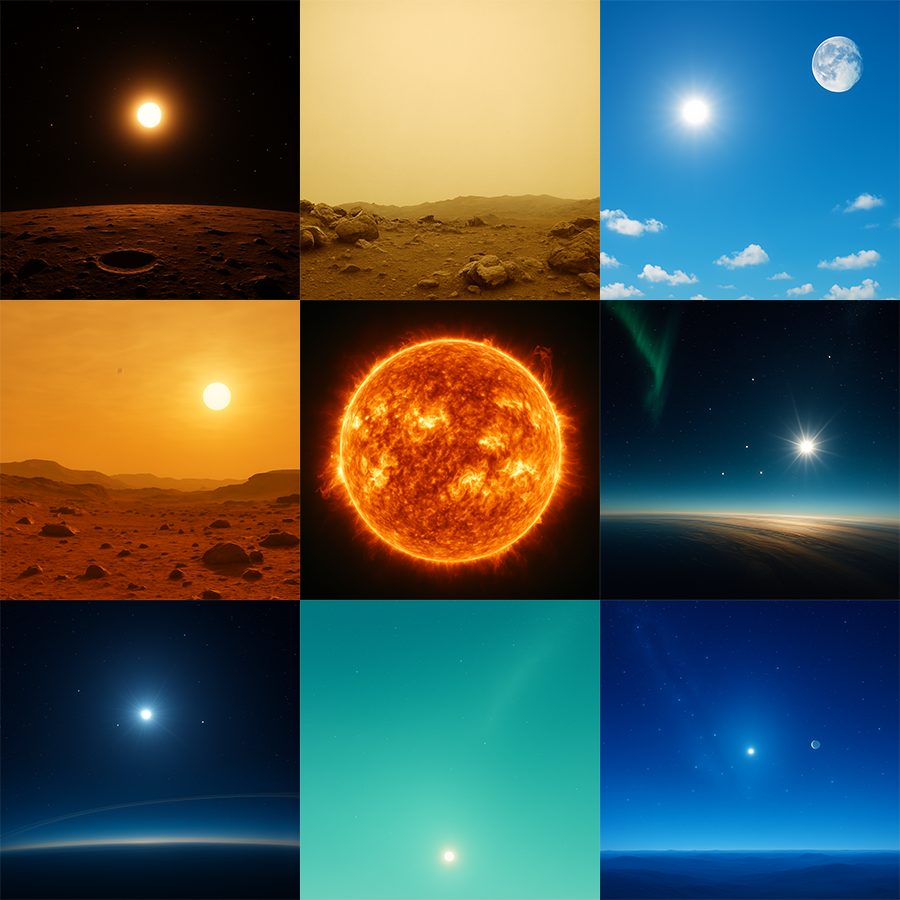
\includegraphics[width=0.8\textwidth]{27_PlanetarySkyColors/SKIES.png}\\
    {Nine simulated daytime skies from each planet in the Solar System, arranged heliocentrically around the Sun in a 3$\times$3 grid. The rows (left to right, top to bottom) correspond to: Mercury, Venus, Earth; Mars, Sun, Jupiter; Saturn, Uranus, Neptune. Each panel reflects sky color, atmospheric scattering, and visible celestial features such as moons, rings, and the Sun's apparent size, as modeled for surface or high-atmosphere observation.
    }   
\end{center}